% Copyright 2026  Ed Bueler

\documentclass[10pt,
               svgnames,
               hyperref={colorlinks,
                         citecolor=DeepPink4,
                         linkcolor=FireBrick,
                         urlcolor=blue},
               usepdftitle=false]{beamer}

\usetheme{Madrid}
\usecolortheme{beaver}
\setbeamercovered{transparent}
\setbeamerfont{frametitle}{size=\large}
\setbeamercolor*{block title}{bg=red!10}
\setbeamercolor*{block body}{bg=red!5}

\usepackage[english]{babel}
\usepackage[latin1]{inputenc}
\usepackage{times}
\usepackage[T1]{fontenc}
% Or whatever. Note that the encoding and the font should match. If T1
% does not look nice, try deleting the line with the fontenc.

\usepackage{fancyvrb,empheq,bm,xspace,dsfont,esint}
%\usepackage{minted}
\usepackage{tikz}
\usetikzlibrary{positioning,arrows.meta}

% If you wish to uncover everything in a step-wise fashion, uncomment
% the following command: 
%\beamerdefaultoverlayspecification{<+->}

\newcommand{\bb}{\mathbf{b}}
\newcommand{\bc}{\mathbf{c}}
\newcommand{\bbf}{\mathbf{f}}
\newcommand{\bl}{\bm{\ell}}
\newcommand{\bn}{\mathbf{n}}
\newcommand{\br}{\mathbf{r}}
\newcommand{\bs}{\mathbf{s}}
\newcommand{\bx}{\mathbf{x}}
\newcommand{\by}{\mathbf{y}}
\newcommand{\bv}{\mathbf{v}}
\newcommand{\bu}{\mathbf{u}}
\newcommand{\bw}{\mathbf{w}}

\newcommand{\bE}{\mathbf{E}}
\newcommand{\bV}{\mathbf{V}}

\newcommand{\cB}{\mathcal{B}}
\newcommand{\cE}{\mathcal{E}}
\newcommand{\cM}{\mathcal{M}}
\newcommand{\cR}{\mathcal{R}}

\newcommand{\bzero}{\bm{0}}

\newcommand{\CC}{\mathbb{C}}
\newcommand{\NN}{\mathbb{N}}
\newcommand{\RR}{\mathbb{R}}
\newcommand{\ZZ}{\mathbb{Z}}

\newcommand{\one}{\mathds{1}}

\newcommand{\Div}{\nabla\cdot}
\newcommand{\grad}{\nabla}

\newcommand{\range}{\operatorname{range}}
\newcommand{\Span}{\operatorname{span}}

\newcommand{\Matlab}{\textsc{Matlab}\xspace}
\newcommand{\eps}{\epsilon}

\newcommand{\ds}{\displaystyle}

\newcommand{\ip}[2]{\left<#1,#2\right>}

\newcommand{\twovect}[4]{\ensuremath{{#1}_{#2} =
                            \begin{bmatrix} #3 \\ #4 \end{bmatrix}}}

\newcommand{\rbullet}{{\color{FireBrick} \bullet}}

\newcommand*\circled[1]{\tikz[baseline=(char.base)]{
            \node[shape=circle,draw,inner sep=2pt] (char) {#1};}}

\newcommand{\textbook}{Saxe, \emph{Beginning Functional Analysis}}

\DefineVerbatimEnvironment{mVerb}{Verbatim}{numbersep=2mm,
frame=lines,framerule=0.1mm,framesep=2mm,xleftmargin=4mm,fontsize=\scriptsize}

\newcommand{\itemnum}[1]{\setcounter{enumi}{#1}\usebeamertemplate{enumerate item}}



\title{Fundamental theorems of calculus, integration-by-parts, and weak derivatives}

\subtitle{calculations for week 9}

\author{Ed Bueler}

\institute[]{UAF Math 617 Functional Analysis}

\date{Spring 2026}


\begin{document}
\beamertemplatenavigationsymbolsempty

\begin{frame}
  \maketitle
\end{frame}


\begin{frame}{Outline}
  \tableofcontents[hideallsubsections]
\end{frame}

\AtBeginSection[]
{% do not put toc here this time
}


\section{the fundamental theorem of calculus in $\RR^1$}

\begin{frame}{indefinite integral of an $L^1$ function}

\begin{itemize}
\item for $a<b$ real numbers, recall that
	$$L^1([a,b]) = \Big\{f:[a,b]\to\RR\,\big|\,f \text{ is measurable and } \int_a^b |f(x)|\,dx <\infty\Big\}$$

    \begin{itemize}
    \item[$\circ$] remember this is actually a \emph{lie}; the elements of $L^1$ are \emph{equivalence classes} up to almost everywhere
    \end{itemize}
\item what happens when you integrate $f\in L^1$ to get a new function?
	$$F(x) = \int_a^x f(t)\,dt$$

    \begin{itemize}
    \item[$\circ$] this is an \emph{indefinite integral}
    \end{itemize}
\item does the fundamental theorem of calculus (FTC) apply?
	$$\frac{d}{dx}\left(\int_a^x f(t)\,dt\right) \stackrel{?}{=} f(x)$$

    \begin{itemize}
    \item[$\circ$] is $F'(x)=f(x)$?
    \end{itemize}
\end{itemize}
\end{frame}


\begin{frame}{fundamental theorem of calculus (FTC)}

\begin{theorem}[easy direction]
If $f\in L^1([a,b])$ then $F(x) = \int_a^x f(t)\,dt$ is continuous, and it is differentiable almost everywhere, and $F'=f$ almost everywhere.
\end{theorem}

\only<1>{
\noindent picture of proof:

\vspace{57mm}
}
\only<2>{
\begin{proof}[{\small Proof \alert{when we also assume $f$ is continuous}}]
{\footnotesize
If $f\in C([a,b])$ then bounded: $|f|\le M$.  Let $\eps>0$.  If $|x-y|<\delta=\frac{\eps}{M}$, and $x<y$, then
	$$|F(x)-F(y)| = \left|\int_x^y f(t)\,dt\right| \le \int_x^y |f(t)|\,dt \le M |x-y| < M\delta = \eps,$$
so $F$ is continuous.  Since $f$ is continuous at $x$ then there is $\gamma=\gamma(x)>0$ so that $|f(t)-f(x)|<\eps$ if $|t-x|<\gamma$.  Choose any $0<h<\gamma$.  Then
\begin{align*}
\left|\frac{F(x+h)-F(x)}{h} - f(x)\right| &= \left|\frac{1}{h} \int_x^{x+h} f(t)\,dt -  \frac{1}{h} \int_x^{x+h} f(x)\,dt\right| \\
&\le \frac{1}{h} \int_x^{x+h} |f(t)-f(x)|\,dt < \frac{1}{h} \int_x^{x+h} \eps\,dt = \eps
\end{align*}
(A similar argument handles $-\gamma<h<0$.)  This shows $f(x)=\lim_{h\to 0} \frac{F(x+h)-F(x)}{h}$; in particular the two-sided limit exists at every $x$.
}
\end{proof}
}
\end{frame}


\begin{frame}{how the integral is well-behaved when $f\in L^1$}

\begin{lemma}[``absolute continuity of the Lebesgue integral'']
Suppose $f\in L^1([a,b])$ and $\eps>0$.  There exists $\delta>0$ so that if $m(E)<\delta$ then
	$$\int_E |f|\,dm < \eps.$$
\end{lemma}

\begin{proof}[{\small Proof.}]
{\footnotesize
Let $g_k = \min\{|f|, k\}$.  This defines a sequence $0\le g_k \le |f|$ so that $g_k \nearrow |f|$, but where $0 \le g_k \le k$ so $g_k$ is bounded.  By the Monotone Convergence Theorem,
    $$\int_{[a,b]} |f|\,dm = \lim_{k\to\infty} \int_{[a,b]} g_k\,dm$$
Given $\epsilon > 0$, choose $K$ large enough that $\int_{[a,b]} (|f| - g_K)\,dm < \epsilon/2$.  Then for any measurable $E \subset [a,b]$:
    $$\int_E |f|\,dm = \int_E g_K\,dm + \int_E (|f| - g_K)\,dm \le \int_E K\,dm + \int_{[a,b]} (|f| - g_K)\,dm \le K \cdot m(E) + \frac{\epsilon}{2}$$
Now set $\delta = \eps/(2K)$. If $m(E) < \delta$ then $\int_E |f|\,dm < \eps$.
}
\end{proof}
\end{frame}


\begin{frame}{picture of the absolute continuity of the Lebesgue integral}

\noindent picture:

\vspace{70mm}
\end{frame}


\begin{frame}{classical definition of absolute continuity}

\begin{definition}
a continuous function $f:[a,b]\to\RR$ is \emph{absolutely continuous} if for all $\eps>0$ there is $\delta>0$ so that if we have a finite collection of disjoint intervals $[\alpha_i,\beta_i]$, with total length less than $\delta$:
	$$\sum_{i=1}^n (\beta_i - \alpha_i) <\delta,$$
then the variation of $f$ on those intervals is less than $\eps$:
	$$\sum_{i=1}^n |f(\alpha_i) - f(\beta_i)| < \eps$$
\end{definition}
\end{frame}


\begin{frame}{picture of absolute continuity}

\noindent picture:

\vspace{70mm}
\end{frame}


\begin{frame}{flavors of continuity for $f:[a,b]\to\RR$}

\begin{center}
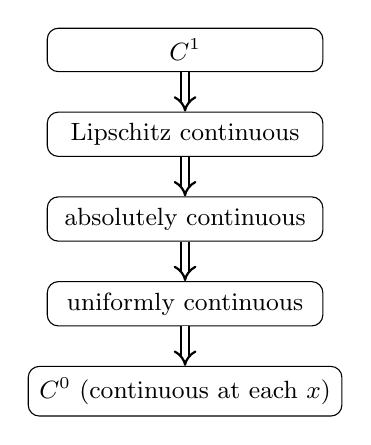
\begin{tikzpicture}[node distance=0.5cm,
    box/.style={draw, rounded corners, align=center,
                inner sep=4pt, minimum width=3.5cm, font=\small},
    impl/.style={-{Implies}, double, double distance=2pt, thick}]
\node[box] (C1)  {$C^1$};
\node[box, below=of C1]  (Lip) {Lipschitz continuous};
\node[box, below=of Lip] (AC)  {absolutely continuous};
\node[box, below=of AC]  (UC)  {uniformly continuous};
\node[box, below=of UC]  (C)   {$C^0$ (continuous at each $x$)};
\draw[impl] (C1) -- (Lip);
\draw[impl] (Lip) -- (AC);
\draw[impl] (AC) -- (UC);
\draw[impl] (UC) -- (C);
\end{tikzpicture}
\end{center}

\medskip
\begingroup
\setbeamerfont{block title}{size=\normalsize}
\begin{definition}
\small
a continuous function $f:[a,b]\to\RR$ is \emph{Lipschitz continuous} if there is $L\ge 0$ so that
	$$|f(x)-f(y)| \le L|x-y|$$
for all $x,y\in [a,b]$
\end{definition}
\endgroup
\end{frame}


\begin{frame}{the Fundamental Theorem of Calculus again}

\begin{theorem}[FTC 1]
If $f\in L^1([a,b])$ then $F(x) = \int_a^x f(t)\,dt$ is \alert{absolutely continuous}, and it is differentiable almost everywhere, and $F'=f$ almost everywhere.
\end{theorem}

\begin{proof}[{\small sketch of the proof}]
{\footnotesize
Approximate $f$ in $L^1$ by a continuous function $g$.  Show that the difference $f-g$, which can be large, can't be large on a big set.  (Vitali covering lemma.)  Conclude.
}
\end{proof}

\begin{theorem}[FTC 2]
If $F(x)$ is absolutely continuous then $f=F'$ exists a.e.~and $f\in L^1$ and $F(x)-F(a) = \int_a^x f(t)\,dt$ for all $x$.
\end{theorem}

\bigskip
\begin{itemize}
\item take-home message: if $f\in L^1$ then its indefinite integral $F(x) = \int_a^x f(t)\,dt$ is a nice ``very'' continuous function which is differentiable a.e.
\item \emph{and} you can recover $f$ from $F$ by differentiating, at least a.e.
\end{itemize}
\end{frame}


\begin{frame}{\emph{not the FTC}, part 1: continuity is necessary \dots}

\medskip \noindent \emph{question}: if $F:[a,b]\to\RR$ is differentiable almost everywhere ($f=F'$ a.e.), and if $f\in L^1$, then is it true that
    $$F(x) -F(a)= \int_a^x f(t)\,dt \quad \text{for all } x\in [a,b]?$$

\medskip \noindent \emph{answer}: \alert{no}

\bigskip
\noindent picture:

\vspace{17mm}

\noindent \hrulefill

{\small
\begin{itemize}
\item my pair of formulas with $F'(x) = G'(x)$ a.e.:
	$$F(x) = \begin{cases} x, & 0<x<1 \\ 2, & 1<x<2\end{cases} \qquad G(x) = \begin{cases} x, & 0<x<1 \\ 1, & 1<x<2\end{cases}$$
    $$F'(x) = G'(x) = \begin{cases} 1, & 0<x<1 \\ 0, & 1<x<2\end{cases}$$
\end{itemize}
}
\end{frame}


\begin{frame}{\emph{not the FTC}, part 2: but not sufficient (the devil's staircase)}

\medskip \noindent \emph{question}: if $F:[a,b]\to\RR$ is continuous, and if $f=F'$ exists almost everywhere, and if $f\in L^1$, then is it true that
    $$F(x) -F(a)= \int_a^x f(t)\,dt \quad \text{for all } x\in [a,b]?$$

\medskip \noindent \emph{answer}: also \alert{no}!

\bigskip
\noindent picture:

\vspace{50mm}
\end{frame}


\begin{frame}{final conclusion: Lebesgue's FTC in 1D}

\begin{block}{Fundamental Theorem of Calculus}
\begin{enumerate}
\item If $f \in L^1([a,b])$ then $F(x) = \int_a^x f(t)\,dt$ is in $AC([a,b])$,\footnote{We define $AC([a,b])=(\text{absolutely continuous functions on } [a,b])$.} and it is differentiable a.e., and
    $$\frac{d}{dx}\left(\int_a^x f(t)\,dt\right) = f(x)$$
for almost every $x$.
\item If $F \in AC([a,b])$ then $f=F'$ exists a.e., and $f\in L^1([a,b])$, and
    $$F(x)-F(a) = \int_a^x f(t)\,dt$$
for all $x$.
\end{enumerate}
\end{block}


\end{frame}


% at start of sections 2,3,... put outline
\AtBeginSection[] {
    \begin{frame}{Outline}
    \setbeamertemplate{section in toc}[sections numbered]
    \tableofcontents[currentsection]%,hideallsubsections]
    \end{frame}
}


\section{divergence theorem on $\RR^d$}

\begin{frame}{divergence theorem in the plane $\RR^2$}

\begin{theorem}[divergence theorem \dots as a Green's theorem]
Suppose $\Omega\subset\RR^2$ is bounded and open.  Suppose that the curve $C=\partial \Omega$ is continuously-differentiable, and orient it counter-clockwise.  If $u(x,y)$ and $v(x,y)$ are continuously-differentiable functions on $\overline{\Omega}$ then
	$$\iint_\Omega u_x + v_y \,dx\,dy = \oint_{C} u\, dy - v\, dx.$$
\end{theorem}

{\small
\begin{itemize}
\item the right side is a \emph{curve (line) integral}; we must parameterize $C$ as $(x(t),y(t))$:
  $$\oint_{C} u\, dy - v\, dx = \int_0^T u(x(t),y(t)) y'(t) - v(x(t),y(t)) x'(t)\,dt$$
\item pictures (with disconnected and not-simply-connected possibilities):

\vspace{25mm}
\end{itemize}
}
\end{frame}


\begin{frame}{divergence theorem in the plane $\RR^2$}

\begin{theorem}[divergence theorem]
Suppose $\Omega\subset\RR^2$ is bounded and open, and $\partial \Omega$ is continuously-differentiable.  Let $\bn$ be the outward normal along $\partial \Omega$.  If $\bV$ is a continuously-differentiable vector field on $\overline{\Omega}$ then
	$$\int_\Omega \Div \bV\,dm = \int_{\partial\Omega} \bV\cdot \bn\,ds$$
\end{theorem}

\begin{itemize}
\item $\bV=\bV(x,y)$ has components $\bV=\ip{u}{v}$
\item \alert{$\Div \bV = u_x + v_y$} is the \emph{divergence} of the vector field
\item I will just use ``$\int$'' instead of $\iint$, $\oint$, etc.
\item $dm$ is Lebesgue measure in $\RR^2$
\item $ds$ is (induced submanifold) Lebesgue measure along the 1D curve $\partial\Omega$
    \begin{itemize}
    \item[$\circ$] nontrivially defined! use parameterized boundary, Jacobian determinant, \dots
    \end{itemize}
\end{itemize}
\end{frame}


\begin{frame}{divergence theorem example}

\begin{block}{Example}
Let $\Omega = \{(x,y)\,:\,x^2+y^2<1\}$ be the unit disk.  Then $\partial\Omega$ is the unit circle.  Let $\bV=\left<x,y+1\right>$.  Is it true?
	$$\int_\Omega \Div \bV\,dm \stackrel{?}{=} \int_{\partial\Omega} \bV\cdot \bn\,ds$$
\end{block}

\noindent solution steps:
\begin{itemize}
\item<2> parameterize $\partial\Omega$:\, $(x(t),y(t))=(\cos(t),\sin(t))$, $0\le t \le 2\pi$
\item<2> $\bn=\ip{x}{y}=\ip{\cos(t)}{\sin(t)}$
\item<2> $ds=dt$ (arclength parameterized)
\item<2> $\bV\cdot \bn = \left<x,y+1\right> \cdot \ip{x}{y} = x^2 + y^2 + y = 1 + \sin(t)$
\item<2> $\Div \bV = 1 + 1 = 2$
\item<2> thus (\emph{no surprise!}) the two sides are equal:
\begin{align*}
\int_\Omega \Div \bV\,dm &= \int_\Omega 2\,dm = 2 \pi\\
\int_{\partial\Omega} \bV\cdot \bn\,ds &= \int_0^{2\pi} 1 + \sin(t)\,dt = 2\pi
\end{align*}
\end{itemize}
\end{frame}


\begin{frame}{divergence theorem in $\RR^d$}

\begin{itemize}
\item there is nothing intrinsically two-dimensional about the theorem!
\end{itemize}

\begin{theorem}[divergence theorem]
Suppose $\Omega\subset\RR^d$ is bounded and open, and $\partial \Omega$ is continuously-differentiable or Lipschitz.  Let $\bn$ be the outward normal along $\partial \Omega$.  If $\bV$ is a continuously-differentiable vector field on $\overline{\Omega}$ then
	$$\int_\Omega \Div \bV\,dm = \int_{\partial\Omega} \bV\cdot \bn\,ds$$
\end{theorem}

\begin{itemize}
\item<2> $dm$ is Lebesgue measure in $\RR^d$
\item<2> $ds$ is $(d-1)$-dim'l Lebesgue measure (submanifold measure)
\item<2> a point $x\in\RR^d$ has \emph{coordinates} $x_i$: \quad $x = (x_1,\dots,x_d)$
\item<2> a vector field $\bV:\Omega \to \RR^d$ has \emph{components}, $\bV = \left<v_1,\dots,v_d\right>$, and the components are scalar functions, $v_k = v_k(x_1,\dots,x_d)$
\item<2> the \emph{divergence} of the vector field is
	$$\Div \bV = \frac{\partial v_1}{\partial x_1} + \dots + \frac{\partial v_d}{\partial x_d} = \sum_{k=1}^d \frac{\partial v_k}{\partial x_k}$$
\end{itemize}
\end{frame}


\begin{frame}{picture of divergence theorem in $\RR^3$ (and hints of proof)}

picture in $\RR^3$:

\vspace{70mm}
\end{frame}


\begin{frame}{most-famous usage in physics}

{\small
\begin{itemize}
\item Gauss' law for electric fields might look like this in a physics text.
\end{itemize}

\begin{block}{Gauss' law (``integral form'')}
Suppose $\bE:\RR^3\to\RR^3$ is the (continuously-differentiable) electric field.  Suppose $\Omega \subset \RR^3$ is a bounded domain with smooth boundary $\partial\Omega$.  Then
	$$\boxed{\only<1>{\oiint_{\partial\Omega}}\only<2>{\int_{\partial\Omega}} \bE \cdot \bn \,ds = \frac{Q}{\eps_0}}$$
where $Q$ is the net enclosed charge within $\Omega$, and $\eps_0>0$ is a constant.
\end{block}

\begin{itemize}
\item apply the divergence theorem on the left, and write $Q$ as the integral of a charge density function $\rho:\RR^3\to\RR$, $\rho \in L^1$:
	$$\int_\Omega \Div \bE \,dm = \frac{1}{\eps_0} \int_\Omega \rho\,dm$$
\item since this applies over any $\Omega\subset \RR^3$, we get Gauss' law in ``PDE form'':
	$$\boxed{\Div \bE = \frac{\rho}{\eps_0}}$$
\end{itemize}
}
\end{frame}


\begin{frame}{fundamental theorems in any dimension}

\begin{itemize}
\item the Fundamental Theorem of Calculus, in any dimension, says that the integral of a derivative can be computed by integrating over the boundary:
    $$\int_\Omega d\omega = \int_{\partial\Omega} \omega \qquad \text{\alert{\emph{(Stokes theorem)}}}$$

    \begin{itemize}
    \item[$\circ$] making this precise requires defining \emph{chains} $\Omega$ and \emph{differential forms} $\omega$
    \item[$\circ$] which I'm not going to do
    \end{itemize}
\item a stack of Fundamental Theorems for $\Omega\subset\RR^d$, in various dimensions:
\begin{align*}
\int_a^b F'\,dm &= F(b)-F(a) &&\text{\footnotesize (interval domain, two-point boundary)} \\
\iint_\Omega \Div \bV\,dm &= \oint_{\partial\Omega} \bV\cdot \bn\,ds &&\text{\footnotesize (planar domain, closed-curve boundary)} \\
\iiint_\Omega \Div \bV\,dm &= \oiint_{\partial\Omega} \bV\cdot \bn\,ds &&\text{\footnotesize (solid domain, closed-surface boundary)} \\
\int_\Omega \Div \bV\,dm &= \int_{\partial\Omega} \bV\cdot \bn\,ds &&\text{\footnotesize ($\RR^d$ domain, $(d-1)$-dim'l closed boundary)}
\end{align*}
\end{itemize}
\end{frame}


\section{integration by parts (in $\RR^1$ and in $\RR^d$)}


\begin{frame}{product rule and integration-by-parts in $\RR^1$}

\begin{itemize}
\item this is very familiar!
\item suppose $f(x),g(x)$ are continuously-differentiable {\small (or absolutely continuous)}
\item then:
	$$\Big(f(x) g(x)\Big)' = f'(x) g(x) + f(x) g'(x)$$
\item if we integrate both sides from $a$ to $b$, and apply FTC on left:
	$$\Big[f(x) g(x)\Big]_a^b = \int_a^b f'(x) g(x)\,dx + \int_a^b f(x) g'(x)\,dx$$
\item rearranging, we get integration-by-parts:\footnote{also known as $\int u\,dv = u\,v - \int v\,du$, but then you put in limits of integration \dots}
	$$\boxed{\int_a^b f(x) g'(x)\,dx = \Big[f(x) g(x)\Big]_a^b - \int_a^b f'(x) g(x)\,dx}$$
\item it suffices for $f,g$ to be absolutely continuous (and thus $f',g'\in L^1$)
\end{itemize}
\end{frame}


\begin{frame}{product rules in $\RR^d$}

\begin{itemize}
\item notation:
    \begin{itemize}
    \item[$\circ$] $x\in\RR^d$ has coordinates: \quad $x = (x_1,\dots,x_d)$
    \item[$\circ$] $f,g:\RR^d\to\RR$ are scalar functions
    \item[$\circ$] $\bV$ has components: \quad $\bV = \left<v_1,\dots,v_d\right>$ \quad where $v_k$ are scalar functions
    \item[$\circ$] gradient $\grad f = \left<\frac{\partial f}{\partial x_1}, \dots,\frac{\partial f}{\partial x_d}\right>$ and divergence $\Div \bV = \sum_{k=1}^d \frac{\partial v_k}{\partial x_k}$
    \end{itemize}
\item there are \alert{2 priority product rules} in $\RR^d$ to know:\footnote{there are also product rules for the curl (``$\nabla\times\bV$''), and/or for the exterior derivative and differential-forms wedge product (``$d$'' and ``$\omega\wedge\nu$''); know these for electricity and magnetism!}

\begin{block}{product rule 1: partial derivatives (of scalar functions)}
    $$\frac{\partial}{\partial x_k} \Big(f \,g\Big) = \frac{\partial f}{\partial x_k} g + f \frac{\partial g}{\partial x_k}$$
\end{block}

\begin{block}{product rule 2: divergence/gradient}
    $$\Div (f\,\bV) = \grad f\cdot \bV + f\,\Div \bV$$
\end{block}
\end{itemize}
\end{frame}


\begin{frame}{integration-by-parts in $\RR^d$}

\begin{itemize}
\item the \alert{2 priority integration-by-parts rules} in $\RR^d$ come from the two product rules \dots via the same logic as in $\RR^1$!
\item the first rule is simplest and most useful \emph{when the boundary integral is zero}, thus the assumption of compact support
\item because of the assumption of compact support, the boundary of $\Omega$ is allowed to be weird

\begin{block}{integration-by-parts 1: partial derivatives}
if $\Omega\subset\RR^d$ is open, and if $f,g\in C_c^1(\Omega)$ then
    $$\int_\Omega \frac{\partial f}{\partial x_k} g\,dm = -\int_\Omega f \frac{\partial g}{\partial x_k}\,dm$$
\end{block}
\end{itemize}
\end{frame}


\begin{frame}{nice functions}

\begin{itemize}
\item but what is ``$C_c^1(\Omega)$''?
\end{itemize}

\begin{definition}
\begin{itemize}
\item If $\Omega\subset\RR^d$ is open, we say that a function $f:\Omega\to\RR$ \emph{has compact support} if
	 $$\operatorname{supp}(f) = \{x\in\Omega\,:\,f(x)\ne 0\}$$
is a compact subset of $\Omega$.
\item $C_c(\Omega) = \left\{\text{$\RR$-valued continuous functions which have compact support}\right\}$
\item $C_c^n(\Omega) = \left\{f\in C_c(\Omega)\,:\,\text{partial derivatives up to order $n$ are in } C_c(\Omega)\right\}$
\item $C_c^\infty(\Omega) = \left\{f\in C_c(\Omega)\,:\,\text{partial derivatives of all orders are in } C_c(\Omega)\right\}$
\end{itemize}
\end{definition}

\begin{itemize}
\item note $C_c^0(\Omega)=C_c(\Omega)$
\item \alert{$C_c^\infty(\Omega)$ functions are the nicest}!  you can differentiate and/or integrate over $\Omega$ as much as you want
\end{itemize}
\end{frame}


\begin{frame}{integration-by-parts in $\RR^d$}

\begin{itemize}
\item the second formula, easily derived from the divergence theorem, is sometimes called a \emph{Green's identity} or similar
\item it requires the boundary to have a normal direction, so the boundary cannot be too weird

\begin{block}{integration-by-parts 2: divergence/gradient}
if $\Omega\subset\RR^d$ is open, bounded, and has continuously-differentiable or Lipschitz boundary, and if $f$ and the components of $\bV$ are in $C^1(\overline{\Omega})$, then
    $$\int_\Omega f\,\Div \bV\,dm = \int_{\partial\Omega} f\,\bV\cdot \bn\,ds - \int_\Omega \grad f\cdot \bV\,dm$$
\end{block}
\end{itemize}
\end{frame}


\begin{frame}{compact support and integration-by-parts}

\noindent pictures (partial derivative version on left, divergence/gradient on right):

\vspace{60mm}
\end{frame}


\section{weak derivatives}

\begin{frame}{y}

FIXME start from $(fg)_{x_k} = f_{x_k} g + f g_{x_k}$

\begin{itemize}
\item y
\end{itemize}
\end{frame}


\section{where this is going: Sobolev spaces to solve PDEs}

\begin{frame}{y}

\begin{itemize}
\item y
\end{itemize}
\end{frame}


\section{lecture content in weeks 10 \& 11}

\begin{frame}{lecture content in weeks 10 \& 11}

\begin{itemize}
\item part of this material is only from these slides

\begin{block}{to know from slides:}
\begin{itemize}
\small
\item Lebesgue's FTC on $[a,b]$, with $f\in L^1$ and $F \in AC$
\item divergence theorem in $\RR^d$
\item integration-by-parts in $\RR^d$
\item multi-index notation for derivatives in $\RR^d$, and definition of $C_c^\infty(\Omega)$
\item weak derivative in $\RR^d$
\item Sobolev space $H^1$
\end{itemize}
\end{block}

\item \dots but part will be from Chapter 5 in Saxe, sections 5.1 and 5.2
\end{itemize}

\begin{block}{to define:}
\begin{itemize}
\small
\item linear operator
\item bounded linear operator
\item operator norm
\item dual space \quad (\emph{I will add this closely-related topic})
\end{itemize}
\end{block}
\end{frame}


\begin{frame}{lecture content in weeks 10 \& 11}

\begin{block}{to prove:}
\begin{itemize}
\item a linear operator is continuous if and only if it is bounded (Theorem 5.2)
\item the bounded linear operators $\cB(X,Y)$ form a normed vector space under operator norm (Theorem 5.3)
\item if $Y$ is complete then $\cB(X,Y)$ is complete (Theorem 5.4)
\item the dual space is a Banach space
\item dual vectors on a Hilbert space can be represented by elements of the Hilbert space (Riesz representation theorem)
\end{itemize}
\end{block}

\begin{itemize}
\item Assignment 6 is posted at \quad  \href{https://bueler.github.io/fa/index.html}{\texttt{bueler.github.io/fa}}
\end{itemize}
\end{frame}

\end{document}
